%第4章:検証
%結果(実験で起こったこと)を書く.客観的に.グラフあればなおよし.


\section{検証}

\subsection{単体テスト}

V字モデルに従い,詳細設計の要件を満たしているかどうかを確認する.まず,各種センサが要件を満たすか否かを検証した.次に,各種センサのテスト項目に従い,単体テストを行った.単体テストの第一段階として,確認内容の頭に*印のついていないテスト項目の機能テストを行った.*印のついているテスト項目についてはLEDの点灯に関するものであり,追加を優先する機能ではないと判断し,第二段階のテストに含めた.


\subsection*{Webカメラ}


Webカメラの単体テストを表\ref{t_web}に示す.


\begin{table}[htbp]
\centering
\caption{Webカメラの単体テスト}
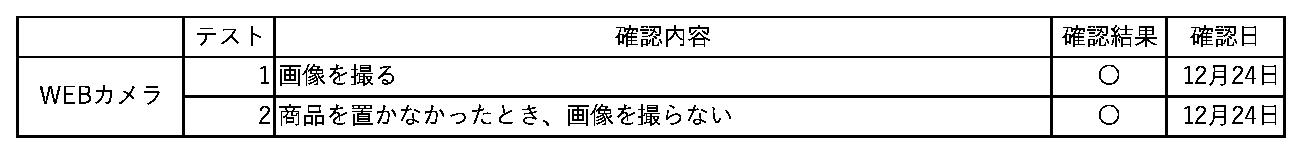
\includegraphics[width = 15cm]{./picture/tantai_web.eps}
\label{t_web}
\end{table}

まず,表\ref{webcamera}における項目1のテストを行った.対象商品をカメラから100mm,150mm,200mmと離し,バーコードを読み取りが可能か,テストをした.カゴの高さが240mmかつ,Webカメラの設置場所はカゴの上部否かを90mmのため,150~200mm程度までバーコードが認識できれば要件を満たすとする.

はじめに,WebカメラとしてロジクールC270を使用し,テストを行った.しかしながら,全ての画像のピントが合っておらず,バーコードを読み取ることができなかった.より画質が高く,ピントの合いやすいスマートフォンのカメラで撮影した動画でバーコード読み取りを試したところ,100mm,150mm程度まで読み取ることができたため,バーコード読み取りシステムの不具合ではなかったことが判明した.画素数もしくはピントを合わせる機能が問題になっていると仮定した.

次に,Raspberry Pi カメラモジュール V2を使用し,テストを行った.Raspberry Pi カメラモジュール V2については画素数はロジクールC270の約6.6倍の画素数のため,もし画素数に問題があるならば判明すると考えた.Raspberry Pi カメラモジュール V2をテストしたところ,ロジクールC270と同じようにピントが合わず,バーコードを読み取ることができなかった.

画素の問題でないことが判明したため,オートフォーカスモデルのロジクールC615を使用しテストを行った.バーコードの読み取り距離について要求を満たしたため,表\ref{jissou}に最終的な実装環境として記載したとおり,ロジクールウェブカメラC615を実装環境とした.項目2においても要求を満たしたことを確認した.


\subsection*{超音波センサ}

超音波センサの単体テストを表\ref{t_chou}に示す.


\begin{table}[htbp]
\centering
\caption{超音波センサの単体テスト}
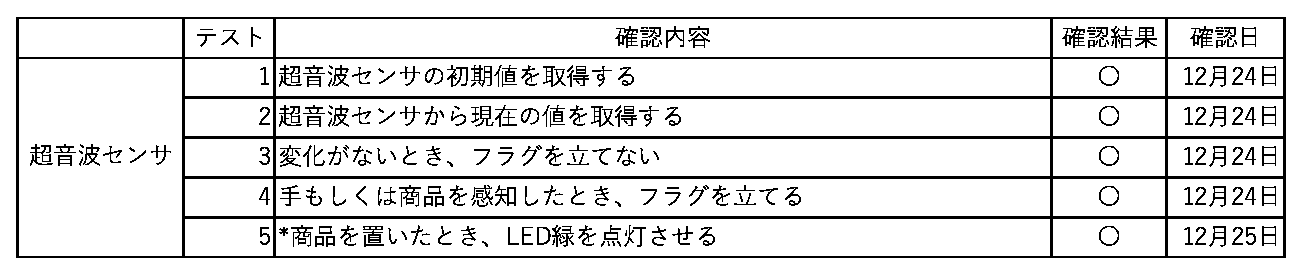
\includegraphics[width = 15cm]{./picture/tantai_chou.eps}
\label{t_chou}
\end{table}

最初に,超音波センサが正しく反応しているか,要求を満たしているかテストを行った.要求としてはカゴの横幅360mmなので,360mm以内を10mm程ずつ測ることができるかどうか確認した.超音波センサは正しく反応し,360mm以上の距離を1mmより小さい距離ずつ測ることができ,要求を満たした.

次に,第一段階の機能テストを行い,機能項目を満たしたことを確認した.同様に,第二段階の機能テストを行い,機能項目を満たしたことを確認した.

\subsection*{ロードセル}

ロードセルの単体テストを表\ref{t_rodoseru}に示す.


\begin{table}[htbp]
\centering
\caption{ロードセルの単体テスト}
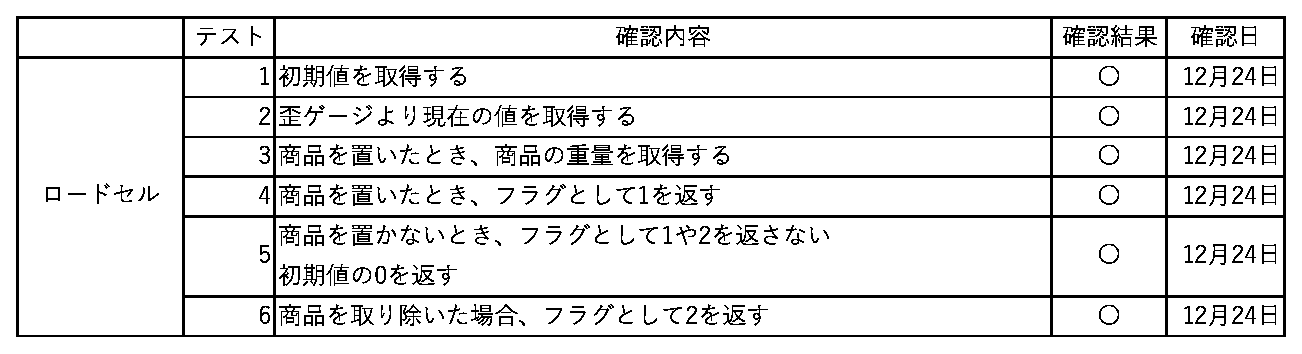
\includegraphics[width = 15cm]{./picture/tantai_rodo.eps}
\label{t_rodoseru}
\end{table}

ロードセルが正しく反応しているか,要求を満たしているかテストを行った.要求として,重量の増減を確認できるか,3kgまでの重量を1g程ずつはかることができるかどうか確認した.ロードセルは正しく反応し,対象商品を1gより小さい値ずつ測ることができた.そのためロードセルは要求を満たした.


\subsection*{データ送信}

データ送信における単体テストを表\ref{t_data}に示す.


\begin{table}[htbp]
\centering
\caption{データ送信の単体テスト}
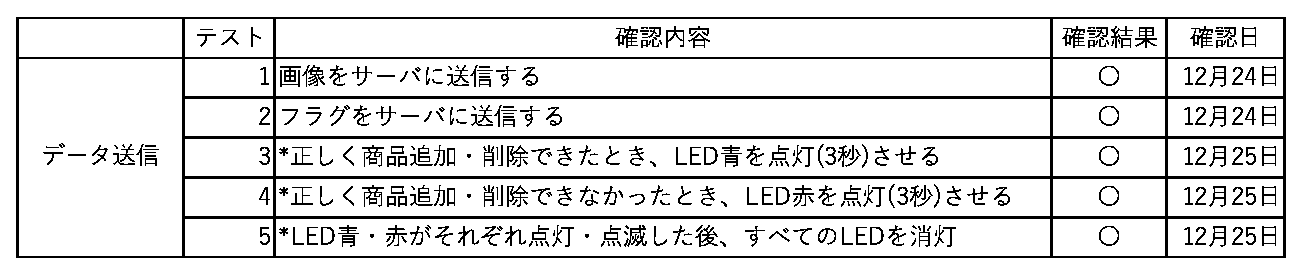
\includegraphics[width = 15cm]{./picture/tantai_data.eps}
\label{t_data}
\end{table}

第一段階の機能テストを行い,機能項目を満たしたことを確認した.同様に,第二段階の機能テストを行い,機能項目を満たしたことを確認した.


\subsection{結合テスト}


V字モデルに従い,基本設計の要件を満たしているか否かを確認する.各実装対象の結合テストを表\ref{t_ketsugo}に示す.


\begin{table}[htbp]
\centering
\caption{結合テスト}
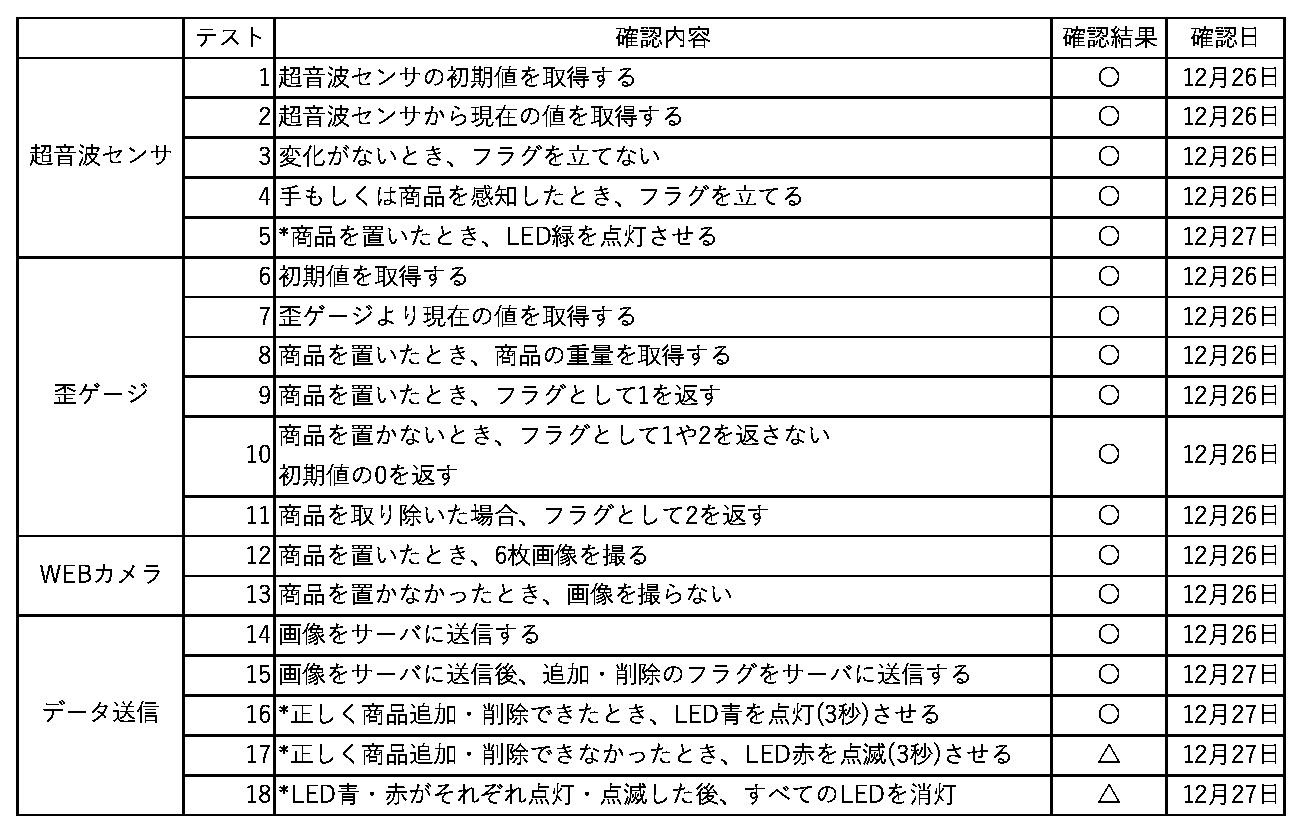
\includegraphics[width = 15cm]{./picture/t_ketsugo.eps}
\label{t_ketsugo}
\end{table}

結合テストの際も,*印以外のテスト項目の機能テストを第一段階として行った.テスト項目14,15の画像をサーバに送信する際,Webカメラから撮影した画像とフラグをセットする順番について問題があった.超音波センサが反応するタイミングとロードセルが反応するタイミングが固定ではなく,どちらが先になるかが予想できなかった.画像とフラグをセットにしてデータを送信する際,画像が先に届くか,フラグが先に届くかが決まっている必要があったため画像とフラグをセットにする方法について考慮する必要があった.解決策として,フラグをキューへ追加し,画像撮影後,画像を画像用の配列へ追加,その後キューからフラグを取り出し,画像の後にフラグを入れセットにして送信する方法を採用した.画像を撮影後,キューが空の場合はフラグがたつまで一定時間待機することとした.上記方法で再度テストを行ったところ,正しく動作を確認した.

次に,*印を含める第二段階のテストを行った.テスト項目17のLEDの点滅について,点灯のほうがテストの際に確認がしやすかったため,項目17は点滅ではなく点灯として動作を確認した.テスト項目18においては,LED赤・青が誤作動し,複数回点灯することがあったため△とした.しかしながら,実際にユーザに正しく情報を伝えることができており,比較的優先度の低いテスト項目だったため,そのまま総合テストへ移行した.


\subsection{総合テスト}


V字モデルに従い,要求分析を満たしているかどうかを確認する.各実装対象のシナリオに基づいた総合テストを表\ref{t_sogo}に示す.


\begin{table}[htbp]
\centering
\caption{総合テスト}
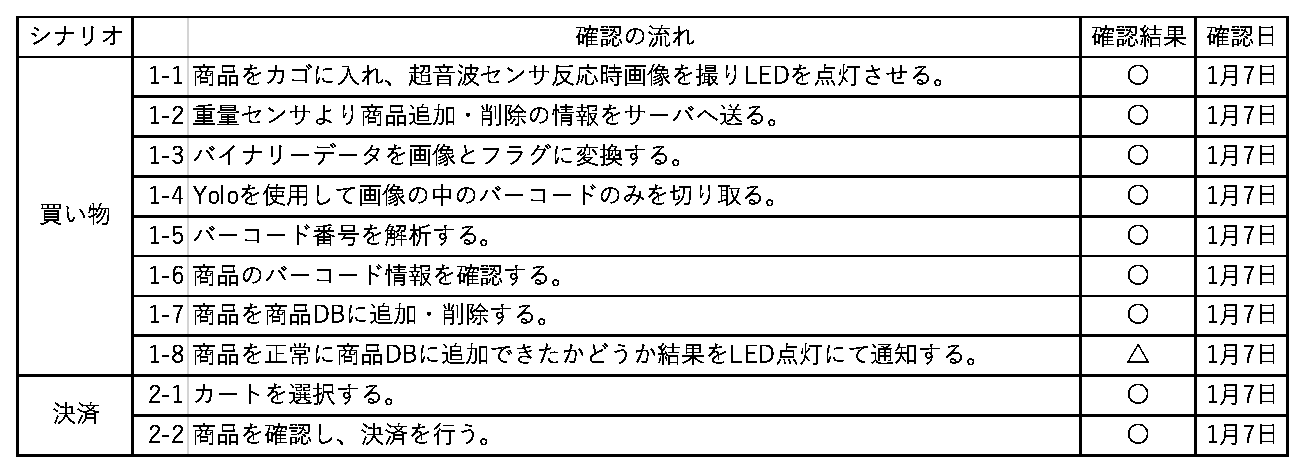
\includegraphics[width = 15cm]{./picture/t_sogo.eps}
\label{t_sogo}
\end{table}

総合テストでは,3.1節の表\ref{sina}のシナリオに沿って動作しているかを確認する.テスト項目1-8においては,LED点灯の誤作動が度々あったため△とした.しかしながら,ユーザに通知するべき情報は正しく通知できていることを確認した.また,シナリオの流れも含め,表\ref{sogo}を確認した.
